\documentclass[class=report,crop=false, 12pt]{standalone}
\usepackage[screen]{../scratch}

\begin{document}

\newcommand{\hexa}{\text{hex}}


\titre[E]{\'Enigmes sur feuilles}
%===============================



%------------------------------------
%\section*{Feuilles 1-2-3}

\begin{enigme}[Premiers pas]

Je me déplace sur la grille en suivant le chemin :

    \centerline{\mot{E E N N O O O N O O S S S E S S}}

Malheureusement, je ne sais plus depuis quelle case je suis parti !

\myfigure{0.9}{
  \tikzinput{eg_premiers_pas}
}  

 
\bigskip

\textbf{Question.} 
Quelle sera la case d'arrivée ?


On rappelle les règles du jeu : 

\emph{  
Je me déplace sur des cases en suivant des instructions Nord, Sud, Est et Ouest.
Pour savoir quelle sera la case suivante, je regarde l'instruction écrite dans la case où je me trouve :
\begin{itemize}
  \item si je suis sur une case \mot{N}, ma prochaine case sera celle située juste au Nord de ma case actuelle,
  \item si je suis sur une case \mot{S}, je me déplacerai d'une case vers le Sud,
  \item pour un case \mot{E}, je me déplacerai vers l'Est,
  \item pour une case \mot{O}, je me déplacerai vers l'Ouest.
\end{itemize}
}


%\begin{solution}
%Réponse : la case B1 (en partant de D3).
%\myfigure{0.8}{
%  \tikzinput{sol_premiers_pas}
%}  
%\end{solution}


\end{enigme}




\begin{enigme}[Répéter]

Nous avons trois couleurs, chacune codée par son initiale : \mot{R} pour rouge, \mot{V} pour vert et \mot{B} pour bleu. Mais ici les couleurs sont codées par trois lettres \mot{X}, \mot{Y} ou \mot{Z}.

\centerline{\mot{Z \  2Y \  2(X 2Y Z) \  2Z \ X \  2(Y 2Z)}}

Sachant qu'il y a plus de rouge que de bleu et plus de bleu que de vert, retrouve quelles sont les couleurs associées à \mot{X}, \mot{Y} et \mot{Z} et colorie les bulles suivantes.

\myfigure{0.9}{
\tikzinput{repeter20}
} 
 
\bigskip

\textbf{Question.} Quelles sont les couleurs des quatre premières bulles ?
\emph{Répondre sous la forme de quatre lettres. Par exemple : \mot{BVRR} pour bleu, vert, rouge, rouge.}


%\begin{solution}
%Réponse : \mot{RBBV}.
%
%\mot{X} = \mot{V} \quad \mot{Y}=\mot{B} \quad \mot{Z}=\mot{R}
%
%\myfigure{0.5}{
%  \tikzinput{sol_repeter}
%}  
%\end{solution}

\end{enigme}



\begin{enigme}[Opérations algébriques I]


Je pars d'un entier $x$ positif et j'effectue successivement les opérations suivantes :
    \begin{itemize}
      \item $x \leftarrow x-3$
      \item $x \leftarrow x \times x$ 
      \item $x \leftarrow x - 27$
    \end{itemize}

Avec l'entier $x$ que j'ai choisi, j'obtiens comme résultat mon entier de départ !
 
\bigskip

\textbf{Question.} Quelle est la valeur de l'entier positif $x$ positif que j'ai choisi ?

%\begin{solution}
%Réponse : $x=9$.
%
%Vérifions que $x=9$ marche.
%    \begin{itemize}
%      \item $x \leftarrow x-3$, maintenant $x$ vaut $9-3$ donc vaut $6$.
%      \item $x \leftarrow x \times x$ , maintenant $x$ vaut $6 \times 6$, donc vaut $36$.
%      \item $x \leftarrow x - 27$, et enfin $x$ vaut $36-27$ donc vaut $9$ !
%    \end{itemize}
%   
%\end{solution}

\end{enigme}


%------------------------------------
%\section*{Feuilles 4-5-6}


\begin{enigme}[Vrai et faux]

Les lampes numérotées 1, 2, 3 et 4 peuvent être allumées ou éteintes, ce qui allume ou éteint les deux lampes du bas.

\myfigure{1}{
  \tikzinput{eg_vraifaux}
}  
 
\bigskip

\textbf{Question.} Quelles lampes faut-il allumer en haut, de sorte que les deux lampes du bas soient allumées en même temps ?
\emph{On indiquera la réponse par la position des lampes à allumer en haut. Par exemple s'il faut allumer les lampes $1$, $3$ et $4$ alors la réponse est $134$.}

%\begin{solution}
%Réponse : $14$ (lampes $1$ et $4$). 
%\end{solution}

\end{enigme}


\begin{enigme}[Opérations algébriques II]

Dans cet exercice, on travaille avec une mini-calculatrice qui ne prend en compte que seulement $5$ chiffres pour la mantisse ($1$ chiffre avant la virgule et $4$ chiffres après).  

Par exemple, si $x = 12,3456$ alors ce nombre est stocké dans la mini-calculatrice sous la forme $nf(x) = 1,2345e1$. Note que le $6$ n'est plus présent.
 
\bigskip

Soit $a = \frac{1286}{9}$ et $b = \frac{1000}{7}$.
On veut calculer la quantité :
$$x = \frac{1}{a-b}.$$

Le premier ordinateur fait des calculs exacts en mémoire, mais affiche seulement une valeur tronquée à $5$ chiffres, c'est-à-dire qu'il calcule :
$$x_1 = nf\left( \frac{1}{a-b} \right).$$

Le second ordinateur tronque les résultats à chaque étape des calculs, c'est-à-dire qu'il calcule :
$$nf(a) \  \text{ et } \  nf(b) \quad \text{puis} \quad 
nf\big( nf(a) - nf(b) \big)$$
et enfin 
$$x_2 = nf \left( \frac{1}{nf\big( nf(a) - nf(b) \big)}\right).$$


\textbf{Question.} Combien vaut $x_2-x_1$ (arrondi à l'entier le plus proche) ?

%
%\begin{solution}
%Réponse : $2$.
%
%\begin{itemize}
%  \item $x_1 = 31.500$
%  \item $nf(a)=$, $nf(b) = $, $nf( nf(a)-nf(b) ) = $,
%  $x_2 = nf() = $
%  \item $x_2-x_1 = 1.83$
%\end{itemize}
%\end{solution}

\end{enigme}



\begin{enigme}[Si ... alors ...]

On a les instructions suivantes :

\begin{center}
\begin{minipage}{0.3\textwidth}
$n \leftarrow \ ?$ \\
$x \leftarrow n$ \\
répéter $n$ fois : \\
\indentation si $x$ est pair, alors : \\ 
\indentation\indentation $x \leftarrow x - 3$ \\
\indentation sinon : \\
\indentation\indentation $x \leftarrow 2\times x + 2$
\end{minipage}
\end{center}

\bigskip

\textbf{Question.} Quelle doit être la valeur de $n$, de sorte qu'à la fin la valeur de $x$ soit $100$ ?

%\begin{solution}
%Réponse : $n=7$.
%\end{solution}

\end{enigme}



%------------------------------------
%\section*{Feuilles 7-8-9}


\begin{enigme}[Boucles I]

Voici un algorithme sous forme de diagramme.
 
\myfigure{0.8}{
\footnotesize\tikzinput{eg_boucles1}
}  
\bigskip

\textbf{Question.} Lorsque la valeur en entrée est $n=10$, quelle est la valeur de $S$ en sortie ?

%\begin{solution}
%Réponse : $70$.
%\end{solution}

\end{enigme}



\begin{enigme}[Chercher et remplacer]

Soit le groupe de lettres :

\centerline{[mrc]?!a[lts]}

et la liste de mots :

\centerline{\mot{malin}\qquad\mot{radis}\qquad\mot{spirale}\qquad\mot{crise}\qquad\mot{miracle}}

\centerline{\mot{classe}\qquad\mot{miette}\qquad\mot{casser}\qquad\mot{amour}\qquad\mot{toujours}}
 
 \centerline{\mot{rail}\qquad\mot{cercle}\qquad\mot{crasse}\qquad\mot{chouette}\qquad\mot{caramel}}
 
\bigskip

\textbf{Question.} Dans cette liste, combien de mots admettent le groupe de lettres proposé ?

%\begin{solution}
%Réponse : 6. Liste : \mot{crise}, \mot{miracle}, \mot{miette}, \mot{casser}, \mot{rail}, \mot{crasse}.
%\end{solution}

\end{enigme}


\begin{enigme}[Puissances de 2]

J'ai une ramette de papier de $5$ cm d'épaisseur qui contient $500$ feuilles.
Je prends une seule feuille.

\begin{itemize}
  \item \emph{Étape 1.} Je plie ma feuille en deux.
  \item \emph{Étape 2.} Je replie ma feuille en deux.
  \item \ldots
  \item \emph{Étape 20.} Je replie une dernière fois ma feuille en deux.
\end{itemize}
    
\bigskip

\textbf{Question.} Quelle est l'épaisseur totale de ma feuille pliée ?
\emph{Répondre en cm, arrondi à l'entier inférieur ou supérieur.}


%\begin{solution}
%Réponse : $\frac{1}{100} \times 2^{20} = 10485,76$ cm, donc réponse est $10485$ ou $10486$.
%\end{solution}

\end{enigme}

%------------------------------------
%\section*{Feuilles 10-11-12}


\begin{enigme}[Binaire]

On travaille avec des nombres en écriture binaire à 7 chiffres (par exemple :
$0.0.1.0.1.1.0$).

On introduit deux opérations sur les nombres binaires à 7 chiffres.
\begin{itemize}
  \item La \emph{négation} qui change chaque $0$ en $1$ et chaque $1$ en $0$.
  Par exemple :
  $$\text{NON}(0.0.1.0.1.1.0) = 1.1.0.1.0.0.1$$

 \item La \emph{multiplication chiffre à chiffre}, avec la règle
 $0 \otimes 0 = 0$ ; $1 \otimes 0 = 0$ ; $0 \otimes 1 = 0$ et $1 \otimes 1 = 1$.
 Pour deux nombres $a$ et $b$ à plusieurs chiffres on applique cette règle entre le premier chiffre de $a$ et le premier chiffre de $b$, puis entre le second chiffre de $a$ et le second chiffre de $b$\ldots Par exemple :
 
\myfigure{1}{
\tikzinput{eg_binaire}
}  
\end{itemize}

\bigskip

Pour cette énigme : 
\begin{itemize}
  \item je pars de $a= 108$ et $b=89$ en écriture décimale,
  \item j'écris $a$ et $b$ en écriture binaire,
  \item je calcule $a \otimes b$,
  \item puis $\text{NON}(a\otimes b)$.
\end{itemize}
 
\bigskip

\textbf{Question.} Quel est l'entier obtenu ? Donner la réponse en écriture décimale.

%\begin{solution}
%Réponse : $55$, car $a = 1101100$, $b = 1011001$,
%$a \otimes b = 1001000$, $\text{NON}(a\otimes b) = 0110111 = 55$.
%\end{solution}

\end{enigme}



\begin{enigme}[Boucles II]

%\myfigure{1}{
%  \tikzinput{}
%}  
 
\textbf{But :} Le programme suivant affiche si un entier $n$ positif ou nul est pair ou impair. Malheureusement les lignes ont été mélangées !

  
\begin{center}
\begin{minipage}{0.8\textwidth}
\textbf{1.}\indentation Sinon:\\
\textbf{2.}\indentation Tant que $n\ge4$:\\
\textbf{3.}\indentation Si (($n=1$) ou  ($n=3$)):\\
\textbf{4.}\indentation\indentation Afficher "Ce nombre est pair."\\
\textbf{5.}\indentation\indentation Afficher "Ce nombre est impair."\\
\textbf{6.}\indentation\indentation $n \leftarrow n - 4$\\
\end{minipage}
\end{center}   
 
\bigskip

\textbf{Question.} Remets les lignes dans l'ordre. \emph{La réponse est la suite des numéros de ligne dans le bon ordre, par exemple 532146.}

%\begin{solution}
%Réponse : 263514.
%
%\begin{center}
%\begin{minipage}{0.8\textwidth}
%\textbf{2.}\indentation Tant que $n\ge4$:\\
%\textbf{6.}\indentation\indentation $n \leftarrow n - 4$\\
%\textbf{3.}\indentation Si ((n=1) ou  (n=3)):\\
%\textbf{5.}\indentation\indentation Afficher "Ce nombre est impair."\\
%\textbf{1.}\indentation Sinon:\\
%\textbf{4.}\indentation\indentation Afficher "Ce nombre est pair."\\
%\end{minipage}
%\end{center} 
%\end{solution}

\end{enigme}


\begin{enigme}[Graphe]

En utilisant les pastilles (6 rouge, 4 bleu, 2 vert), colorie les sommets du graphe de sorte que deux sommets reliés par une arête ne soient pas de la même couleur.

\myfigure{1}{
  \tikzinput{eg_graphe}
}  


\bigskip

\textbf{Question.} Quelles sont les couleurs des pastilles du bas ?
\emph{Par exemple si les pastilles du bas (numérotées 1, 2, 3 et 4) sont vert, rouge, bleu, bleu, alors répondre VRBB.}

\bigskip

{\footnotesize Dans ce problème les arêtes peuvent se croiser ! D'après Dorian Mazauric, \href{https://hal.inria.fr/hal-01366804}{\emph{Graphes et Algorithmes - Jeux grandeur nature}}, 2016.}

%\begin{solution}
%Réponse : RVRR.
%
%\myfigure{0.7}{
%  \tikzinput{eg_graphe-correc}
%}  
%
%\end{solution}

\end{enigme}


%
%------------------------------------
%\section*{Feuilles 13-14-15-16}


\begin{enigme}[Bases de données]


Voici un extrait des tables d'un aéroport.

\bigskip

\begin{center}
{\footnotesize

%
% Destination
\begin{minipage}{0.35\textwidth}

\textbf{Table 1 : Destination/Horaire}\\
\emph{Destination et jour du départ.} \\

\begin{tabular}{|l|l|l|} \hline
\textbf{Id.} & \textbf{Destination} & \textbf{Jour} \\ \hline\hline
D1 & Sydney & Lundi \\ \hline
D2 & Vancouver & Jeudi \\ \hline
D3 & Chicago & Samedi \\ \hline
D4 & Moscou & Lundi \\ \hline
D5 & Istanbul & Dimanche \\ \hline
D6 & Rio & Mercredi \\ \hline
D7 & Le Caire & Samedi \\ \hline
D8 & Rome & Mardi \\ \hline
D9 & Shanghai & Jeudi \\ \hline
\end{tabular}
\end{minipage}
\begin{minipage}{0.3\textwidth}
% Avion
\textbf{Table 2 : Avion}\\
\emph{Avion, modèle, capacité.} \\

\begin{tabular}{|l|c|c|} \hline
\textbf{Id.} & \textbf{Modèle}& \textbf{Capacité} \\ \hline\hline
A1 & A330 & 260 \\ \hline
A2 & B737 & 250 \\ \hline
A3 & B777 & 270 \\ \hline
A4 & A320 & 160 \\ \hline
A5 & B747 & 280 \\ \hline
A6 & A380 & 410 \\ \hline
A7 & A319 & 140 \\ \hline
\end{tabular}
\end{minipage}
%
% Destination
\begin{minipage}{0.3\textwidth}

\textbf{Table 3 : Embarquement}\\
\emph{Terminal et porte.} \\

\begin{tabular}{|l|c|c|} \hline
\textbf{Id.} & \textbf{Terminal} & \textbf{Porte} \\ \hline\hline
E1 & 1 & 7 \\ \hline
E2 & 2 & 6 \\ \hline
E3 & 1 & 1 \\ \hline
E4 & 2 & 3 \\ \hline
E5 & 1 & 4 \\ \hline
E6 & 1 & 2 \\ \hline
E7 & 2 & 2 \\ \hline
\end{tabular}
\end{minipage}
}
\end{center}


\bigskip

\begin{center}
{\footnotesize
\textbf{Table 4 : Vol}\\
\emph{Un vol est défini par un avion, une destination et un lieu d'embarquement} \\

\begin{tabular}{|l|l|l|} \hline
\textbf{Id. avion} & \textbf{Id. destination} & \textbf{Id. embarquement}\\ \hline\hline
A3 & D2 & E5 \\ \hline
A7 & D6 & E3 \\ \hline
A6 & D7 & E3 \\ \hline
A1 & D5 & E1 \\ \hline
A3 & D8 & E6 \\ \hline
A4 & D1 & E6 \\ \hline
A2 & D6 & E4 \\ \hline
A6 & D8 & E2 \\ \hline
A6 & D2 & E1 \\ \hline
\end{tabular}
}
\end{center}
 
\bigskip

\textbf{Question.} Sachant que tous les avions sont remplis, combien de personnes au total décolleront du lundi au vendredi, depuis le terminal 1 ?

%\begin{solution}
%Réponse : 1250 (lignes 1,2,5,6,9 de la table 4).
%\end{solution}

\end{enigme}




\begin{enigme}[Pixels]

\sauteligne

\begin{itemize}
  \item On colorie en bleu les pixels du segment $[A_1B_1]$ suivant l'algorithme de Bresenham.
  \item On colorie en rouge les pixels du segment $[A_2B_2]$ suivant l'algorithme de Bresenham.
\end{itemize}


\myfigure{0.8}{
  \tikzinput{eg_pixels}
}  
 
\bigskip

\textbf{Question.} Combien de pixels sont colorés à la fois en bleu et en rouge ?

%\begin{solution}
%Réponse : 4
%
%\myfigure{0.7}{
%  \tikzinput{eg_pixels-correc}
%} 
%
%\end{solution}

\end{enigme}




\begin{enigme}[Diviser pour régner]



Panoramix a concocté une potion magique qu'il a cachée parmi d'autres bouteilles.
Les bouteilles sont numérotées de $0$ à $255$.
Asterix a besoin de retrouver la bouteille, mais n'a pas le temps de les tester une à une car la potion met 24h à agir. Il décide d'appliquer une méthode \og{}diviser pour régner\fg{} :
\begin{itemize}
  \item le gaulois \textbf{0} goûte les bouteilles numéro $0$, $2$, $4$\ldots (il goûte donc une bouteille sur deux) ;
  \item le gaulois \textbf{1} goûte les bouteilles numéro $0$ et $1$, puis $4$ et $5$, puis $8$ et $9$\ldots (il goûte donc deux bouteilles sur quatre) ;
  \item le gaulois \textbf{2} goûte les bouteilles numéro $0$ à $3$,  puis $8$ à $11$\ldots (il goûte donc quatre bouteilles sur huit) ; 
  \item \ldots  
  \item le gaulois \textbf{7} goûte les bouteilles de $0$ à $127$ et pas les suivantes.
\end{itemize}

Après avoir goûté leurs bouteilles, seuls les gaulois \textbf{1}, \textbf{2}, \textbf{4}, \textbf{6} ont des pouvoirs magiques.

%\myfigure{1}{
%  \tikzinput{}
%}  
 
\bigskip

\textbf{Question.} Quel numéro porte la bouteille de potion magique ?


%\begin{solution}
%Réponse : $169$. En effet, les gaulois \textbf{0}, \textbf{3}, \textbf{5}, \textbf{7} n'ont pas de pouvoirs magiques, donc la bouteille porte le numéro
%$n = 2^\mathbf{0}+2^\mathbf{3}+2^\mathbf{5}+2^\mathbf{7} = 169$.
%\end{solution}

\end{enigme}



\begin{enigme}[Couleurs]


Pour transformer une image couleur en une image \og{}noir et blanc\fg{}, on transforme chaque pixel coloré en un pixel en niveau de gris.

\begin{center}
  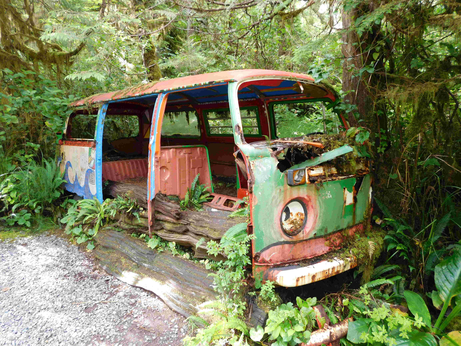
\includegraphics[scale=0.4]{photo_eg_couleurs-color.png}\qquad
  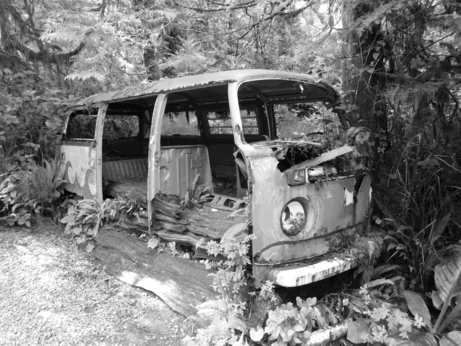
\includegraphics[scale=0.4]{photo_eg_couleurs-grayscale.png}   
\end{center}

Une des formules possibles est :
$$G = 0,21 \times R \  + \  0,72 \times V \  + \  0,07 \times B$$

\begin{itemize}
  \item $R,V,B$ sont les niveaux de rouge, vert et bleu du pixel coloré,
  \item $G$ est le niveau de gris du pixel \og{}noir et blanc\fg{}.
\end{itemize}

Note que, comme l'\oe il humain est plus sensible au vert, la couleur verte a un poids plus important.  
  
\bigskip 
 
 
J'ai une couleur, dont le code RVB en hexadécimal est donné par :
$$R = CE_\hexa \qquad V = B6_\hexa \qquad B = 7D_\hexa$$

\myfigure{1}{
  \tikzinput{eg_couleurs}
}  
 
\bigskip

\textbf{Question.} Quel est le niveau de gris $G$ du pixel \og{}noir et blanc\fg{} ?
Arrondir à l'entier le plus proche et donner la réponse en hexadécimal. \emph{(Par exemple $2A$ ou $D8$\ldots)}

%\begin{solution}
%Réponse : $B7_\hexa = 183$. ($R = 206$, $V = 182$, $B = 125$, $G = 183.05$, $G' = 183 = B7_\hexa$)
%\end{solution}

\end{enigme}

%------------------------------------
%\section*{Feuilles 17-18-19}


\begin{enigme}[Cryptographie]

\definecolor{coul_prive}{rgb}{0.93,0.26,0}
\definecolor{coul_public}{rgb}{0.06,0.63,0}

\newcommand{\prive}[1]{\relax\ifmmode{\color{coul_prive} #1}\else{\bf\color{coul_prive} #1}\fi}
\newcommand{\public}[1]{\relax\ifmmode{\color{coul_public} #1}\else{\bf\color{coul_public} #1}\fi}


Le message suivant a été codé par le chiffre de Vigenère :

\centerline{\public{E GHMYJVP ZEYZ TPYMW VR EYMZTTSL WLUW RSSTYI}}

La clé est composée de $3$ nombres : $\mathbf{(4,\;?\;,7)}$.
Malheureusement j'ai oublié le nombre du milieu !
 
 
\bigskip

\textbf{Question.} Quel est l'entier manquant de la clé qui a codé ce message ?

%\begin{solution}
%Réponse : $11$.
%
%Clé = $(4, 11, 7)$
%
%\public{A VAINCRE SANS PERIL ON TRIOMPHE SANS GLOIRE}
%\end{solution}

\end{enigme}



\begin{enigme}[Triangulation]

Trace la triangulation de Delaunay de cette configuration de points.


\myfigure{1.3}{
  \tikzinput{eg_triangulation_04}  
}

\bigskip

\textbf{Question.} Combien d'arêtes partent des points $A$, $J$ et $M$ ? (Donner la somme des trois entiers)

%\begin{solution}
%Réponse : 17 ($d(A)=4$, $d(J)=7$, $d(M)=6$).
%
%\myfigure{1.1}{
%  \tikzinput{eg_triangulation_05}  
%}
%
%
%\end{solution}

\end{enigme}



\begin{enigme}[Distance entre deux mots]
  
  ~
  
\myfigure{0.7}{
\tikzinput{eg_distance}
} 
\bigskip

\textbf{Question.} Quelle est la distance de Levenshtein entre les mots
\mot{CROCODILE} et \mot{RECTANGLE} ?

%\begin{solution}
%Réponse : 6.
%\end{solution}

\end{enigme}

\end{document}


